\chapter{probability}
\section{general definition}
\begin{itemize}
	\item 对于一个 random variable $x$, 用 $\mathcal{S} = \{x_1, x_2, \cdots\}$ 表示其 possible outcomes.
	
	\item to each event $E \subset \mathcal{S}$ is assigned a probability $p(E)$ that must satisfy:
	\begin{enumerate}
		\item positivity. $p(E) \geq 0$.
		
		\item additivity. $p(A \ \text{or} \ B) = p(A) + p(B), \forall A \cap B = \emptyset$.
		
		\item normalization. $p(\mathcal{S}) = 1$.
	\end{enumerate}
\end{itemize}

\section{one random variable}
\begin{itemize}
	\item 考虑 $\mathcal{S} = \mathbb{R}$.
	
	\item cumulative probability function (CPF) 定义为
	\begin{equation}
		P(y) := \mathrm{prob}(\{x | x < y\}),
	\end{equation}
	那么 $P(- \infty) = 0, P(+ \infty) = 1$, 且 $P(x)$ 是 monotonically increasing.
	
	\item probability density function (PDF) 定义为
	\begin{equation}
		p(x) := \frac{dP}{dx}.
	\end{equation}
	
	\item the expectation value of any function $F(x)$ is
	\begin{equation}
		\braket{F(x)} := \int_{- \infty}^\infty dx \, p(x) F(x).
	\end{equation}
	
	\item 将 $F(x)$ 视为一个 random variable, 那么它的 probability density function 为
	\begin{equation}
		p_F(f) df = \sum_{F(x_i) = f} p(x_i) dx_i \Longrightarrow p_F(f) = \sum_{F(x_i) = f} \frac{p(x_i)}{\big| \frac{dF(x_i)}{dx} \big|}.
	\end{equation}
	
	\noindent\rule[0.5ex]{\linewidth}{0.5pt} % horizontal line
	
	\item the $n$\textsuperscript{th} moment of the PDF is
	\begin{equation}
		m_n := \braket{x^n} = \int_{- \infty}^\infty dx \, x^n p(x).
	\end{equation}
	
	\item the characteristic function is
	\begin{equation}
		\tilde{p}(k) := \braket{e^{- i k x}} = \int dx \, p(x) e^{- i k x},
	\end{equation}
	并有 (Taylor expansion)
	\begin{equation}
		\begin{dcases}
			\tilde{p}(x) = \sum_{n = 0}^\infty \frac{(- i k)^n}{n!} m_n \\
			e^{i k x_0} \tilde{p}(x) = \sum_{n = 0}^\infty \frac{(- i k)^n}{n!} \braket{(x - x_0)^n}
		\end{dcases},
	\end{equation}
	因此 $\tilde{p}(x)$ is the generator of moments.
	
	\noindent\hdashrule[0.5ex]{\linewidth}{0.5pt}{1mm} % horizontal dashed line
	
	\item 类似 moments, 将 cumulants $\braket{x^n}_c$ 定义为
	\begin{equation}
		\ln \tilde{p}(k) = \sum_{n = 1}^\infty \frac{(- i k)^n}{n!} \braket{x^n}_c,
	\end{equation}
	注意到 $\ln(1 + \epsilon) = \sum_{n = 1}^\infty (- 1)^{n + 1} \frac{\epsilon^n}{n}$.
	
	\item 前 4 个 cumulants 分别为
	\begin{equation}
		\begin{dcases}
			\braket{x}_c = \braket{x} & \text{mean} \\
			\braket{x^2}_c = \braket{x^2} - \braket{x}^2 & \text{variance} \\
			\braket{x^3}_c = \braket{x^3} - 3 \braket{x^2} \braket{x} + 2 \braket{x}^3 & \text{skewness} \\
			\braket{x^4}_c = \braket{x^4} - 4 \braket{x^3} \braket{x} - 3 \braket{x^2}^2 + 12 \braket{x^2} \braket{x}^2 - 6 \braket{x}^4 & \text{curtosis}
		\end{dcases}.
	\end{equation}
	
	\item 有
	\begin{equation}
		\frac{\braket{x^n}}{n!} = \sum \Big( \prod_{\{1 \leq m_1 \leq n, 0 \leq m_2 \leq n | \sum m_1 m_2 = n\}} \frac{1}{(m_1!)^{m_2} m_2!} \braket{x^{m_1}}_c^{m_2} \Big).
	\end{equation}
	
	\begin{tcolorbox}[title=calculation:]
		\begin{align}
			\sum_{n = 0}^\infty \frac{(- i k)^n}{n!} \braket{x^n} &= \exp \Big( \sum_{m = 1}^\infty \frac{(- i k)^m}{m!} \braket{x^m}_c \Big) = \prod_{m = 1}^\infty \exp \Big( \frac{(- i k)^m}{m!} \braket{x^m}_c \Big) \notag \\
			&= \prod_{m_1 = 1}^\infty \Big( \sum_{m_2 = 0}^\infty \frac{(- i k)^{m_1 m_2}}{(m_1!)^{m_2} m_2!} \braket{x^{m_1}}_c^{m_2} \Big).
		\end{align}
	\end{tcolorbox}
	
	\item 用 cumulants 表示 moments 的系数 $\frac{n!}{(m_1!)^{m_2} m_2!}$ 可以用一些 graphs 来计算 (cluster expansion), 见 page 39, \textit{Statistical Physics of Particles}, Kardar.
\end{itemize}

\section{some important probability distributions}
\begin{itemize}
	\item the normal (Gaussian) distribution 的 PDF 为
	\begin{equation} \label{A.3.1}
		p(x) = \frac{1}{\sqrt{2 \pi} \sigma} e^{- \frac{(x - \lambda)^2}{2 \sigma^2}},
	\end{equation}
	相应地, characteristic function 为
	\begin{equation}
		\tilde{p}(k) = e^{- i k \braket{x}_c - \frac{k^2}{2} \braket{x^2}_c + \cdots} = e^{- i k \lambda - \frac{k^2 \sigma^2}{2}},
	\end{equation}
	那么
	\begin{equation}
		\braket{x}_c = \lambda, \quad \braket{x^2}_c = \sigma^2, \quad \braket{x^3}_c = \braket{x^4}_c = \cdots = 0.
	\end{equation}
	\begin{itemize}
		\item higher cumulants 消失意味着 cluster expansion 中只含有 one-point and two-point (propagators) clusters.
	\end{itemize}
	
	\item the binomial distribution, $\mathcal{S} = \{A, B\}$, 有
	\begin{equation}
		p_N(N_A) = \begin{pmatrix}
			N \\
			N_A
		\end{pmatrix} p_A^{N_A} (1 - p_A)^{N - N_A}, \quad \begin{pmatrix}
			N \\
			N_A
		\end{pmatrix} = \frac{N!}{N_A! (N - N_A)!},
	\end{equation}
	其 characteristic function 为
	\begin{equation}
		\tilde{p}_N(k) = \sum_{N_A = 0}^N p_N(N_A) e^{- i k N_A} = (p_A e^{- i k} + p_B)^N,
	\end{equation}
	那么
	\begin{equation}
		\braket{N_A}_c = N p_A, \quad \braket{N_A^2}_c = N p_A p_B, \quad \braket{N_A^3}_c = N p_A p_B (1 - 2 p_A), \quad \braket{N_A^4}_c = p_A p_B (1 - 6 p_A + 6 p_A^2).
	\end{equation}
	
	\begin{tcolorbox}[title=calculation:]
		\begin{align}
			\ln \tilde{p}_N(k) =& N \ln(1 + p_A (e^{- i k} - 1)) \notag \\
			=& N \Big( (- i k) p_A + \frac{(- i k)^2}{2} (p_A - p_A^2) + \frac{(- i k)^3}{3!} (p_A - 3 p_A^2 + 2 p_A^3) \notag \\
			& + \frac{(- i k)^4}{4!} (p_A - 7 p_A^2 + 12 p_A^3 - 6 p_A^4) + O(k^5) \Big)
		\end{align}
	\end{tcolorbox}
	
	\begin{itemize}
		\item 可以推广为 multinomial distribution,
		\begin{equation}
			p_N(N_A, N_B, \cdots, N_M) = \frac{N!}{N_A! N_B! \cdots N_M!} p_A^{N_A} p_B^{N_B} \cdots p_M^{N_M}.
		\end{equation}
	\end{itemize}
	
	\item the Poisson distribution 考虑时间长度 $T$ 范围内观察到 $M$ 次衰变的概率 ($dt$ 内发生一次衰变的概率为 $\alpha dt$), 那么
	\begin{equation}
		\begin{dcases}
			p_\lambda(M) = \frac{\lambda^M e^{- \lambda}}{M!} \\
			\tilde{p}_\lambda = e^{\lambda (e^{- i k} - 1)}
		\end{dcases}, \quad \lambda = \alpha T, \quad \text{and} \quad \braket{M^n}_c = \lambda.
	\end{equation}
	\begin{itemize}
		\item the Poisson distribution 的图像如下所示:
		
		\begin{figure}[H]
			\centering
			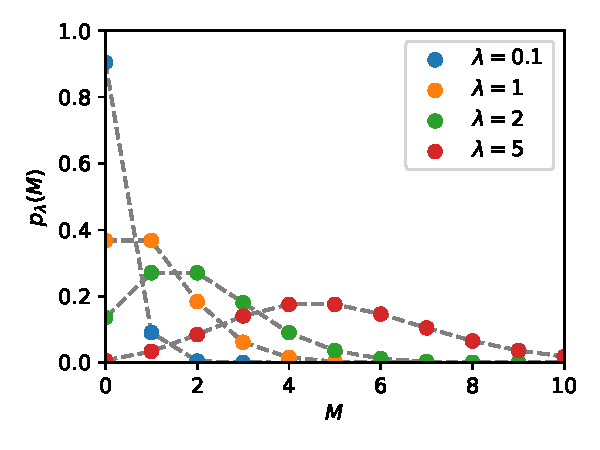
\includegraphics[scale=0.8]{figures/the Poisson distribution.pdf}
			\caption{the Poisson distribution.}
		\end{figure}
	\end{itemize}
	
	\begin{tcolorbox}[title=calculation:]
		参考 binomial distribution, 将 $dt$ 时间内发生一次衰变记为 $A$, 未衰变记为 $B$, 那么
		\begin{equation}
			p_A = \alpha dt, \quad p_B = 1 - p_A, \quad N = \frac{T}{dt}, \quad N_A = M,
		\end{equation}
		因此 ($N \gg 1$)
		\begin{align}
			& \begin{dcases}
				\ln \begin{pmatrix}
					N \\
					M
				\end{pmatrix} \simeq N \ln N - (N - M) \ln(N - M) - M - \ln M! \\
				\ln((\alpha dt)^M (1 - \alpha dt)^{N - M}) = M \ln \frac{\lambda}{N} + (N - M) \ln \Big( 1 - \frac{\lambda}{N} \Big)
			\end{dcases} \notag \\
			\Longrightarrow & \begin{aligned}
				\ln p_\lambda(M) \simeq& \Big( N \ln N - (N - M) \ln(N - M) - M - \ln M! \Big) \\
				& + \Big( M \ln \lambda - M \ln N - \lambda \frac{N - M}{N} \Big) \\
				=& N (\ln N - \ln(N - M)) + M (\ln(N - M) - \ln N) \\
				& - M - \ln M! + M \ln \lambda - \lambda \frac{N - M}{N} \\
				\simeq& M + \frac{M^2}{2 N} - \frac{M^2}{N} - M - \ln M! + M \ln \lambda - \lambda \frac{N - M}{N} \simeq - \ln M! + M \ln \lambda - \lambda
			\end{aligned} \notag \\
			\Longrightarrow & p_\lambda(M) = \frac{\lambda^M e^{- \lambda}}{M!}.
		\end{align}
		
		更简单的方法是计算 $\tilde{p}_\lambda(M)$,
		\begin{equation}
			\tilde{p}_\lambda(M) = \lim_{dt \rightarrow 0} (1 + \alpha dt (e^{- i k} - 1))^N = \lim_{N \rightarrow \infty} \Big( 1 + \frac{\lambda}{N} (e^{- i k} - 1) \Big)^N = e^{\lambda (e^{- i k} - 1)}.
		\end{equation}
	\end{tcolorbox}
\end{itemize}

\section{many random variables}
\begin{itemize}
	\item 考虑 $N$ 个随机变量, 且 $\mathcal{S} = \mathbb{R}^N$.
	
	\item $d^N x$ 体元中的概率用 joint PDF $p(\vec{x})$ 描述, 如果 the $N$ variables are independent, 那么
	\begin{equation}
		p(\vec{x}) = \prod_{i = 1}^N p_i(x_i).
	\end{equation}
	
	\item unconditional PDF 描述 $(x_1, \cdots, x_m)$ 的概率密度, 而剩余的 $(x_{m + 1}, \cdots, x_N)$ 取值任意, 那么
	\begin{equation}
		p(x_1, \cdots, x_m) = \int dx_{m + 1} \cdots dx_N \, p(\vec{x}).
	\end{equation}
	
	\item conditional PDF 描述 $(x_{m + 1}, \cdots, x_N)$ 条件下 $(x_1, \cdots, x_N)$ 的概率密度, 有
	\begin{equation}
		p(x_1, \cdots, x_m | x_{m + 1}, \cdots, x_N) = \frac{p(\vec{x})}{p(x_{m + 1}, \cdots, x_N)}.
	\end{equation}
	
	\item 如果变量独立, 那么 unconditional PDF 等于 conditional PDF.
	
	\item $F(\vec{x})$ 的 expectation value 为
	\begin{equation}
		\braket{F(\vec{x})} = \int d^N x \, p(\vec{x}) F(\vec{x}).
	\end{equation}
	
	\item the joint characteristic function is
	\begin{equation}
		\tilde{p}(\vec{k}) = \braket{e^{- i \vec{k} \cdot \vec{x}}}.
	\end{equation}
	
	\item the joint moments and joint cumulants are generated by $\tilde{p}(\vec{k})$ and $\ln \tilde{p}(\vec{k})$ respectively, as
	\begin{equation}
		\begin{dcases}
			\braket{x_1^{n_1} \cdots x_N^{n_N}} = \frac{\partial^{n_1}}{\partial (- i k_1)^{n_1}} \cdots \frac{\partial^{n_N}}{\partial (- i k_N)^{n_N}} \tilde{p}(\vec{k} = 0) \\
			\braket{x_1^{n_1} \cdots x_N^{n_N}}_c = \frac{\partial^{n_1}}{\partial (- i k_1)^{n_1}} \cdots \frac{\partial^{n_N}}{\partial (- i k_N)^{n_N}} \ln \tilde{p}(\vec{k} = 0)
		\end{dcases},
	\end{equation}
	joint moments 和 joint cumulants 之间依然可以用 cluster expansion 建立关系,
	\begin{equation}
		\frac{\braket{x_1^{n_1} \cdots x_N^{n_N}}}{n_1! \cdots n_N!} = \sum \Big( \prod_{\{1 \leq m_i \leq n_i, 0 \leq l \leq n_i | \sum l m_i = n_i\}} \frac{1}{(m_1! \cdots m_N!)^l l!} \braket{x_1^{m_1} \cdots x_N^{m_N}}_c^l \Big).
	\end{equation}
	
	\begin{tcolorbox}[title=calculation:]
		\begin{align}
			& \sum_{\vec{n}} \frac{(- i k_1)^{n_1} \cdots (- i k_N)^{n_N}}{n_1! \cdots n_N!} \braket{x_1^{n_1} \cdots x_N^{n_N}} \notag \\
			=& \prod_{\vec{m} \neq 0} \exp \Big( \frac{(- i k_1)^{m_1} \cdots (- i k_N)^{m_N}}{m_1! \cdots m_N!} \braket{x_1^{m_1} \cdots x_N^{m_N}}_c \Big) \notag \\
			=& \prod_{\vec{m} \neq 0} \Big( \sum_{l = 0}^\infty \frac{(- i k_1)^{l m_1} \cdots (- i k_N)^{l m_N}}{(m_1! \cdots m_N!)^l l!} \braket{x_1^{m_1} \cdots x_N^{m_N}}_c^l \Big).
		\end{align}
	\end{tcolorbox}
	
	\item 如果 $x_i, x_j$ 互相独立, 那么 $\braket{x_i x_j}_c = \braket{x_i x_j} - \braket{x_i} \braket{x_j} = 0$, (实际上, $\braket{\cdots x_i \cdots x_j \cdots}_c = 0$).
	
	\begin{tcolorbox}[title=calculation:]
		注意到
		\begin{equation}
			\ln \tilde{p}_N(\vec{k}) = \ln \tilde{p}'(\cdots, k_i, \cdots) + \ln \tilde{p}''(\cdots, k_j, \cdots).
		\end{equation}
	\end{tcolorbox}
	
	\item the joint Gaussian distribution 是 \eqref{A.3.1} 的推广, 为
	\begin{equation}
		\begin{dcases}
			p(\vec{x}) = \frac{1}{\sqrt{(2 \pi)^N \det(C)}} \exp \Big( - \frac{1}{2} \sum_{i j} (C^{- 1})_{i j} (x_i - \lambda_i) (x_j - \lambda_j) \Big) \\
			\tilde{p}(\vec{k}) = \exp \Big( - i \vec{k} \cdot \vec{\lambda} - \frac{1}{2} \vec{k} \cdot C \cdot \vec{k} \Big)
		\end{dcases},
	\end{equation}
	其中 $C = C^T$, 那么
	\begin{equation}
		\braket{x_i} = \lambda_i, \quad \braket{x_i x_j}_c = C_{i j}.
	\end{equation}
	\begin{itemize}
		\item 更多结果 (Wick theorem) 参考笔记 \href{https://github.com/siyang03/my-note---A.-Zee-QFT}{A. Zee QFT} 或 \textit{Quantum Field Theory and Critical Phenomena}, Zinn-Justin.
	\end{itemize}
\end{itemize}

\section{sums of random variables and the central limit theorem}
\begin{itemize}
	\item 考虑 $X = \sum_{i = 1}^N x_i$, 那么 $X$ 的 PDF 为
	\begin{align}
		p_X(X) &= \int d^N x \, p(\vec{x}) \frac{d}{dX} \theta(X - \sum_{i = 1}^N x_i) \notag \\
		&= \int d^N x \, p(\vec{x}) \delta(X - \sum_{i = 1}^N x_i) = \int dx_1 \cdots dx_{N - 1} \, p(x_1, \cdots, x_{N - 1}, X - {\textstyle\sum_{i = 1}^{N - 1} x_i}),
	\end{align}
	相应地, the characteristic function 为
	\begin{equation}
		\tilde{p}_X(K) = \braket{e^{- i K \sum_{i = 1}^N x_i}} = \tilde{p}(k_1 = \cdots = k_N = K),
	\end{equation}
	因此, cumulants 为
	\begin{align}
		& \ln \tilde{p}_X(K) = (- i K) \sum_i \braket{x_i}_c + \frac{(- i K)^2}{2!} \sum_{i, j} \braket{x_i x_j}_c + \frac{(- i K)^3}{3!} \sum_{i, j, k} \braket{x_i x_j x_k}_c + \cdots \notag \\
		\Longrightarrow & \braket{X}_c = \sum_i \braket{x_i}_c, \quad \braket{X^2}_c = \sum_{i, j} \braket{x_i x_j}_c, \quad \braket{X^3}_c = \sum_{i, j, k} \braket{x_i x_j x_k}_c, \quad \cdots
	\end{align}
	
	\item the central limit theorem: 如果
	\begin{equation}
		p_N(\vec{x}) = p(x_1) \cdots p(x_N) \quad \text{and} \quad \braket{x^n}_c \ll N^{\frac{n}{2} - 1},
	\end{equation}
	那么, 当 $N \rightarrow \infty$ 时, 有
	\begin{equation}
		\lim_{N \rightarrow \infty} p_X(X) = \frac{1}{\sqrt{2 \pi} \sigma_X} e^{- \frac{(X - \lambda_X)^2}{2 \sigma_X^2}}, \quad \lambda_X = N \braket{x}_c, \quad \sigma_X^2 = N \braket{x^2}_c.
	\end{equation}
	
	\begin{tcolorbox}[title=proof:]
		令
		\begin{equation}
			Y = \frac{X - \braket{X}}{\sqrt{N}} \quad \text{with} \quad \braket{X} = N \braket{x}_c,
		\end{equation}
		那么
		\begin{align}
			p_Y(Y) &= \int d^N x \, p(x_1) \cdots p(x_N) \delta({\textstyle Y + \frac{\braket{X}}{\sqrt{N}} - \frac{1}{\sqrt{N}} \sum_{i = 1}^N x_i}) \notag \\
			&= \int \frac{dq}{2 \pi} e^{i q \big( Y + \frac{\braket{X}}{\sqrt{N}} \big)} \int d^N x \, p(x_1) \cdots p(x_N) e^{- i \frac{q}{\sqrt{N}} \sum_{i = 1}^N x_i} \notag \\
			&= \int \frac{dq}{2 \pi} e^{i q \big( Y + \frac{\braket{X}}{\sqrt{N}} \big)} \tilde{p}^N({\textstyle \frac{q}{\sqrt{N}}}),
		\end{align}
		并注意到 (saddle point integration)
		\begin{equation}
			\tilde{p}(k) = e^{- i k \braket{x}_c + \frac{(- i k)^2}{2} \braket{x^2}_c + \cdots},
		\end{equation}
		因此
		\begin{equation}
			p_Y(Y) = \int \frac{dq}{2 \pi} \exp \Big( i q Y - \frac{q^2}{2} \braket{x^2}_c + O({\textstyle \frac{1}{\sqrt{N}}}) \Big) = \frac{1}{\sqrt{2 \pi \braket{x^2}_c}} e^{- \frac{Y^2}{2 \braket{x^2}_c}}.
		\end{equation}
	\end{tcolorbox}
\end{itemize}
